% !TeX spellcheck = en_GB

\section{Testing}
\label{testing}

In the following chapters we illustrate, how we test our prototype and architecture.

\subsection{Unit Tests}\label{unit-tests}
As we use test driven development (TDD) to develop the prototype, we make heavy use of unit tests. Our Definition of Done\cite{project-plan} states that \emph{reasonable unit and integration tests [must] exist and pass.}

Therefore, these tests are executed on every build run of our continuous integration, that is on every repository push and pull request.


\subsection{Integration Tests}\label{integration-tests}
Our integration tests are split into two main environments: A minimal one as defined in Figure \ref{fig:integrationtestsmall} and a medium network, as defined in Figure \ref{fig:integrationtestmedium}.

\begin{figure}
	\centering
	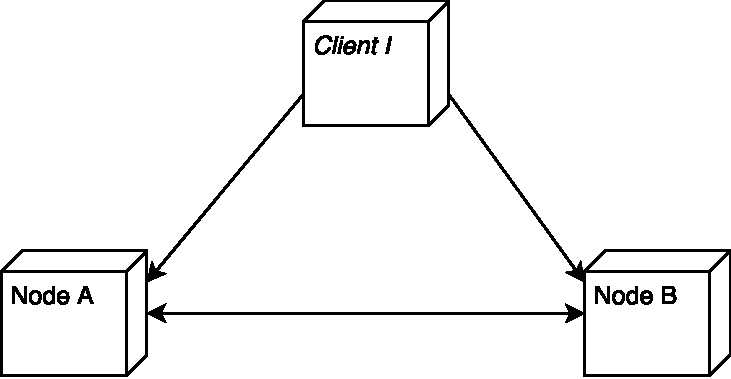
\includegraphics[width=0.5\linewidth]{resources/integration_test_small}
	\caption[Minimal integration test]{Minimal integration test with one client and two nodes.}
	\label{fig:integrationtestsmall}
\end{figure}

\begin{figure}
	\centering
	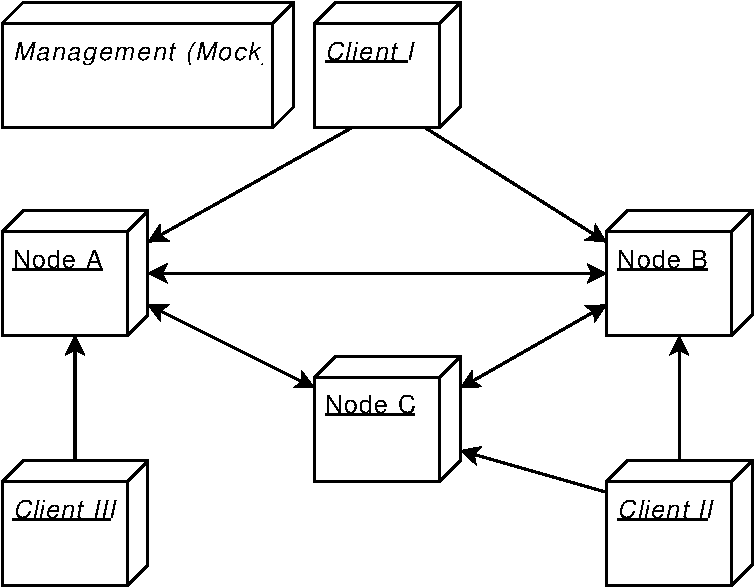
\includegraphics[width=0.5\linewidth]{resources/integration_test_medium}
	\caption[Medium integration test]{Medium integration test with three clients and three nodes.}
	\label{fig:integrationtestmedium}
\end{figure}

These two, rather small nework styles will probably be the most commonly used deployments, yet cover most of the possible problems that may occur.

On these two networks, the implemented scenarios as defined in Appendix \ref{sec:scenarios} are tested (if applicable).

The integration tests are to be run on every tagged release (i.e. at least once every sprint).

\subsubsection{Implementation}

To bootstrap the infrastructure we utilise Docker Compose, a tool for defining and running multi-container Docker applications\cite{docker-compose}. The node application, as well as the client and a managment mockup are run in separate containers, connected over a virtual network.

\subsection{Architecture tests}

Architectural tests are special, manually run tests to verify the scalability of our software architecture.

\subsubsection{Size scalability}
As per our requirements in Appendix \ref{requirements}, the architecture should scale up to 100 nodes. To test this scenario, we use the same underlying techniques as in our integration tests (see chapter \ref{integration-tests}), but scale the infrastructure up to the required limits.

\subsubsection{Network data capacity}
Our requirements (Appendix \ref{requirements}) also state, that a node must be able to handle up to e.g. 2TB of data. To test this requirement, we create large amounts of random data that has to be stored. This is a realistic requirement, as e.g. a compressed image, audio and movie collection might reach such sizes in practice.
